
%%%%%%%%%%%%%%%%%%%%%%% file typeinst.tex %%%%%%%%%%%%%%%%%%%%%%%%%
%
% This is the LaTeX source for the instructions to authors using
% the LaTeX document class 'llncs.cls' for contributions to
% the Lecture Notes in Computer Sciences series.
% http://www.springer.com/lncs       Springer Heidelberg 2006/05/04
%
% It may be used as a template for your own input - copy it
% to a new file with a new name and use it as the basis
% for your article.
%
% NB: the document class 'llncs' has its own and detailed documentation, see
% ftp://ftp.springer.de/data/pubftp/pub/tex/latex/llncs/latex2e/llncsdoc.pdf
%
%%%%%%%%%%%%%%%%%%%%%%%%%%%%%%%%%%%%%%%%%%%%%%%%%%%%%%%%%%%%%%%%%%%


\documentclass[runningheads,a4paper]{llncs}

\usepackage[english, spanish]{babel}
\usepackage[utf8]{inputenc}
\usepackage[T1]{fontenc}
\usepackage{lmodern}
\usepackage{amssymb}
\setcounter{tocdepth}{3}
\usepackage{graphicx}
\usepackage{epstopdf}
\usepackage{float}

\usepackage{url}

\newcommand{\keywords}[1]{\par\addvspace\baselineskip
\noindent\keywordname\enspace\ignorespaces#1}

 \setcounter{secnumdepth}{3}

\begin{document}

\mainmatter  % start of an individual contribution

% first the title is needed
\title{Algoritmos de Búsqueda Multiarranque y Genéticos}

% a short form should be given in case it is too long for the running head
\titlerunning{Algoritmos de Búsqueda Basados en Trayectorias.}

% the name(s) of the author(s) follow(s) next
%
% NB: Chinese authors should write their first names(s) in front of
% their surnames. This ensures that the names appear correctly in
% the running heads and the author index.
%
\author{Alejandro Trujillo Caballero
}
%
\authorrunning{Algoritmos de Búsqueda Basados en Trayectorias..}
% (feature abused for this document to repeat the title also on left hand pages)

% the affiliations are given next; don't give your e-mail address
% unless you accept that it will be published
\institute{Universidad de Huelva. Grado en Ingeniería Informática.}

%
% NB: a more complex sample for affiliations and the mapping to the
% corresponding authors can be found in the file "llncs.dem"
% (search for the string "\mainmatter" where a contribution starts).
% "llncs.dem" accompanies the document class "llncs.cls".
%

\toctitle{}
\tocauthor{Alejandro Trujillo Caballero}
\maketitle

\selectlanguage{spanish}
\begin{abstract}
Análisis del funcionamiento de varios algoritmos de búsqueda multiarranque (GRASP, ILS y VNS) y genéticos aplicados al Problema de Asignación Cuadrática.
\keywords{Búsqueda multiarranque, GRASP, ILS, VNS, Algoritmos Genéticos, Genético CHC, Asignación Cuadrática (QAP).}
\end{abstract}


\section{Introducción}

\subsection{Problema de Asignación Cuadrática}

El Problema de Asignación Cuadrática (QAP) es un problema de optimización combinatoria que consiste en asignar una serie de unidades a localizaciones (teniendo el mismo número de ambas). El objetivo es optimizar una función de coste que consiste en la suma de los productos de la distancia entre localizaciones y el transito entre las unidades asignadas.

 Un ejemplo de aplicación de este problema podría ser la distribución de los diferentes departamentos de un hospital en las diferentes plantas o zonas del edificio.

\section{Algoritmos Analizados}

\subsection{Algoritmo Greedy o Voraz}

Se ha utilizado un algoritmo voraz como base para el análisis del resto de algoritmos.

El algoritmo intenta minimizar el coste asignado las unidades con mayor transito a las localizaciones más céntricas.

El algoritmo siempre sigue el mismo criterio para construir una solución y obtiene la misma por lo que no puede considerase una búsqueda.

\subsection{Métodos Multiarranque}

Los métodos multiarranque se basan en la ejecución de un algoritmo de búsqueda local básico con diferentes soluciones iniciales (generalmente aleatorias) con el objetivo de explorar un espacio de soluciones mayor.

Los algoritmos que se han utilizado son mejoras sobre este planeamiento básico del multiarranque.

\subsubsection{GRASP}
~\\

El algoritmo GRASP intenta mejorar las soluciones iniciales desde las que arrancan las ejecuciones. En cada iteración se genera una solución greedy aleatorizada, a la que se aplica un algoritmo de búsqueda local. Finalmente el algoritmo devuelve la mejor solución encontrada entre todas las ejecuciones.

Para construir la solución greedy aleatorizada se parte de la misma premisa que en el algoritmo greedy normal. Localizaciones y unidades se ordenan según su potencial, pero en lugar de emparejar la mejor localización con la mejor unidad las parejas se van formando eligiendo aleatoriamente una de las \emph{l} primeras localizaciones y una de las \emph{l} primeras unidades.

En nuestro caso, se realizaran 10 iteraciones y el valor del parámetro \emph{l} sera $l = 0.1 \cdot n $ siendo $n$ el tamaño del problema.

\subsubsection{ILS}
~\\

El algoritmo ILS (Iterated Local Search) intenta refinar una solución mediante ejecuciones sucesivas de búsquedas locales junto con un operación de mutación de la solución.

Partiendo de una solución inicial aleatoria el algoritmo aplica una búsqueda local. Una vez obtenida la solución la compara con la mejor solución obtenida hasta ese momento y aplica la mutación a la mejor de las dos. Tras mutar la solución inicia una nueva búsqueda local tomándola como punto de partida.

En nuestro caso la mutación consiste en seleccionar aleatoriamente una sublista dentro de la solución de tamaño $s = n/4 $ donde $n$ es el tamaño del problema y desordenarla de forma aleatoria.

Se aplicaran 10 iteraciones, la primera sobre una solución aleatoria y las 9 restantes sobre la mutación de la mejor solución encontrada.

\subsubsection{VNS}
~\\

La Búsqueda de Entorno Variable o VNS (Variable Neighborhood Search) se basa en la idea de variar el concepto de vecindario dentro de una búsqueda local, aumentando el tamaño de este si la búsqueda no avanza.

El algoritmo parte de una solución aleatoria a la cual aplica una búsqueda local. Una vez obtenido un resultado, aplica una mutación como en el caso del algoritmo ILS y vuelve a aplicar la búsqueda local. Sin embargo, si la solución obtenida tras la búsqueda local que parte de la solución mutada no mejora la mejor solución obtenida hasta el momento, se incrementa el tamaño de la mutación. 

Una vez que se encuentra una mejor solución, el tamaño de la mutación vuelve a fijarse al mínimo. La condición de parada se establece añadiendo un limite al tamaño de la mutación, es decir, si tras $k_{max}$ iteraciones la solución no ha mejorado en ninguna de ellas, el algoritmo se detiene.

Para nuestro caso el parámetro $k_{max} = 5$. La mutación es la misma que en el algoritmo ILS y se varía el tamaño de la sublista siguiendo la regla $s = n/(9-k)$ donde $n$ es el tamaño del problema y $k$ indica el número de iteraciones consecutivas sin mejora. En el momento que $k > k_{max}$ el algoritmo se detiene.

\subsection{Algoritmos Genéticos}

Los algoritmos genéticos son algoritmos de búsqueda, optimización o aprendizaje basados en los conceptos de selección natural y genética.

El concepto básico de algoritmo genético se basa en tener una población (conjunto de soluciones) y que por ``selección natural'' los mejores individuos (soluciones) se reproduzcan o crucen dando lugar a nuevos individuos diferentes o que muten de forma individual. Estos descendientes y mutantes remplazan la población (o una parte de ella) explorando así las posibles soluciones del problema (y preferiblemente mejorandolas).

\subsubsection{Algoritmo Genético Básico}
~\\

El algoritmo genético básico utilizado tiene las siguientes características:

\begin{itemize}
\item \textbf{Modelo Generacional:} En casa iteración del algoritmo se reemplaza la población completa. 
\end{itemize}


\newpage
\section{Resultados}
Para analizar el funcionamiento de los diferentes algoritmos se han utilizado tres ejemplos de diferente tamaño de los cuales se conoce el coste de la solución óptima:

\begin{itemize}
\item \textbf{Tai25b:} 25 lugares y unidades, coste: 344355646.
\item \textbf{Sko90:} 90 lugares y unidades, coste: 115534.
\item \textbf{Tai150b:} 150 lugares y unidades, coste: 498896643.
\end{itemize}

Para analizar los algoritmos se han realizado 10 ejecuciones de cada uno con diferentes semillas para el generador de números aleatorios (ya que todos los algoritmos tiene algún componente aleatorio). 

A continuación se detallan los resultados obtenidos por cada algoritmo.


\begin{table}[H]
\centering
\caption{Costes de las soluciones proporcionadas por el algoritmo de Búsqueda Aleatoria}

\begin{tabular}{c || r | r | r }
Seed & \qquad  tai25 \qquad \quad & \qquad sko90 \qquad & \qquad \qquad tai150 \qquad\\\hline 
1 	& 1173664963 & 142420 & 683423057 \\
2	& 1194390165 & 141814 & 682175843 \\
3	& 1196021141 & 142056 & 682400410 \\
4	& 1201615718 & 141968 & 682907768 \\
5	& 1186447299 & 142246 & 682840264 \\
6	& 1224953864 & 142340 & 683620162 \\
7	& 1178951674 & 142506 & 681266728 \\
8	& 1194823852 & 141922 & 680849383 \\
9	& 1194916409 & 141802 & 681370190 \\
10	& 1199973625 & 141932 & 681353354 \\ \hline \hline
Media & 1194575871 & 142101 & 682220716 \\
Desv. T & 13949407 & 257 & 975284\\
\end{tabular}
\end{table}


\begin{table}[H]
\centering
\caption{Costes de las soluciones proporcionadas por el algoritmo de Búsqueda Local}

\begin{tabular}{c || r | r | r }
Seed & \qquad  tai25 \qquad \quad & \qquad sko90 \qquad & \qquad \qquad tai150 \qquad\\\hline 
1 	& 413373879 & 118426 & 517754022   \\
2	& 454985757 & 117582 & 513947464 		\\
3	& 353465428 & 118702 & 518922684 	\\
4	& 376336066 & 117696 & 520330467 	\\
5	& 411644796 & 118684 & 522055451 	\\
6	& 352048709 & 119516 & 520584440	\\
7	& 398432882 & 117446 & 515304984 	\\
8	& 472936529 & 118182 & 513041392 \\
9	& 459297404 & 119054 & 515305032 \\
10	& 422745919 & 119124 & 519625414 	\\ \hline \hline
Media & 411526737 & 118441 & 517687135\\
Desv. T &42674173 & 705 & 3103204\\
\end{tabular}
\end{table}


\begin{table}[H]
\centering
\caption{Costes de las soluciones proporcionadas por el algoritmo de Enfriamiento Simulado}

\begin{tabular}{c || r | r | r }
Seed & \qquad  tai25 \qquad \quad & \qquad sko90 \qquad & \qquad \qquad tai150 \qquad\\\hline 
1 	& 366621015 & 117626 & 513226444 \\
2	& 371725572 & 117552 & 513322732 \\
3	& 367818611 & 117170 & 514686453 \\
4	& 398264229 & 117824 & 517801729 \\
5	& 416599460 & 117956 & 515247819 \\
6	& 439006905 & 117568 & 515793920 \\
7	& 365491673 & 118028 & 514295612 \\
8	& 406671691 & 118298 & 519586022 \\
9	& 426523708 & 118000 & 524200812 \\
10	& 359474161 & 117208 & 515421269\\ \hline \hline
Media & 391819703 & 117723 & 516358281\\
Desv. T & 29176378 & 365 & 3374897\\
\end{tabular}
\end{table}

\begin{table}[H]
\centering
\caption{Costes de las soluciones proporcionadas por el algoritmo de Búsqueda Tabú}

\begin{tabular}{c || r | r | r }
Seed & \qquad  tai25 \qquad \quad & \qquad sko90 \qquad & \qquad \qquad tai150 \qquad\\\hline 
1 	& 344743823 & 118244 & 512796581 \\
2	& 345675295 & 117972 & 511883040 \\
3	& 395351036 & 117638 & 517545690 \\
4	& 347720408 & 117906 & 512090462 \\
5	& 363961225 & 118210 & 511258562 \\
6	& 346703840 & 117876 & 510626132 \\
7	& 347984063 & 117642 & 512807837 \\
8	& 347684843 & 118342 & 514336213 \\
9	& 346483036 & 118188 & 514097120 \\
10	& 364427055 & 118520 & 511212655\\ \hline \hline
Media & 355073462 & 118054 & 512865429  \\
Desv. T & 15939318 & 295 & 2040887 \\
\end{tabular}
\end{table}

\newpage
\subsection{Comparación de resultados}

\begin{table}[H]
\centering
\caption{Resultados globales de los algoritmos para el problema Tai25}
\begin{tabular}{c || r | r | r | r}
Algoritmo 	& Peor & Media & Mejor & Desv. T. \\ \hline
Óptimo 		& - 	& 344355646	&	-	&	-		\\
Greedy 		& - 	& 734935031	&	-	&	-		\\ \hline
B. Aleatoria &\quad  1224953864 & \quad  1194575871 & \quad 1173664963 & \quad \textbf{13949407} \\
B. Local & 472936529 & 411526737 & 352048709 & 42674173 \\
Enf. Simu & 439006905 & 391819703 & 359474161 & 29176378 \\
B. Tabú & \textbf{395351036} & \textbf{355073462} & \textbf{344743823} & 15939318 \\
\end{tabular}
\end{table}

\begin{figure}[H]
\center
\centerline{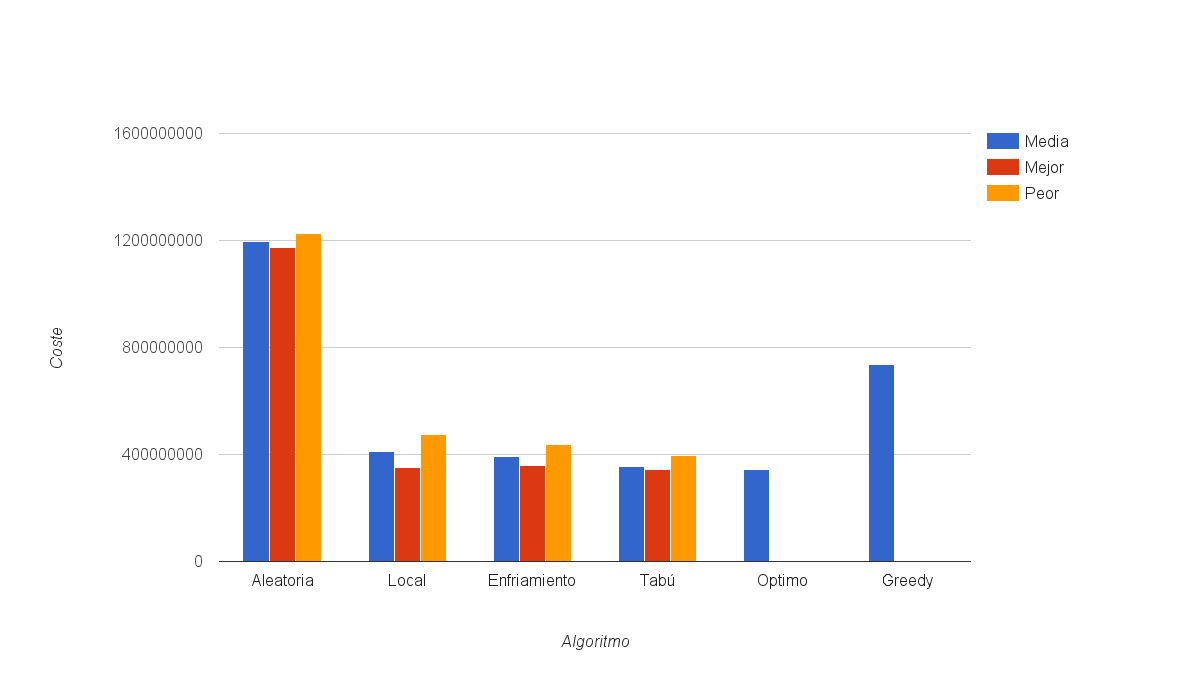
\includegraphics[scale=0.38]{./Grafico25.png}}
\caption{Resultados de los algoritmos para el problema Tai25}
\end{figure}

\begin{table}[H]
\centering
\caption{Resultados globales de los algoritmos para el problema Sko90}
\begin{tabular}{c || r | r | r | r}
Algoritmo 	& Peor & Media & Mejor & Desv. T. \\ \hline
Óptimo 		& - 	& 115534	&	-	&	-		\\
Greedy 		& - 	& 131262	&	-	&	-		\\ \hline
B. Aleatoria & \quad 142506 & \quad 142101 & \quad 141802 & \textbf{257} \\
B. Local & 119516 & 118441 & 117446 & 705 \\
Enf. Simu & \textbf{118298} & \textbf{117723} & \textbf{117170} & 365 \\
B. Tabú & 118520 & 118054 & 117638 & 295 \\
\end{tabular}
\end{table}


\begin{figure}[H]
\center
\centerline{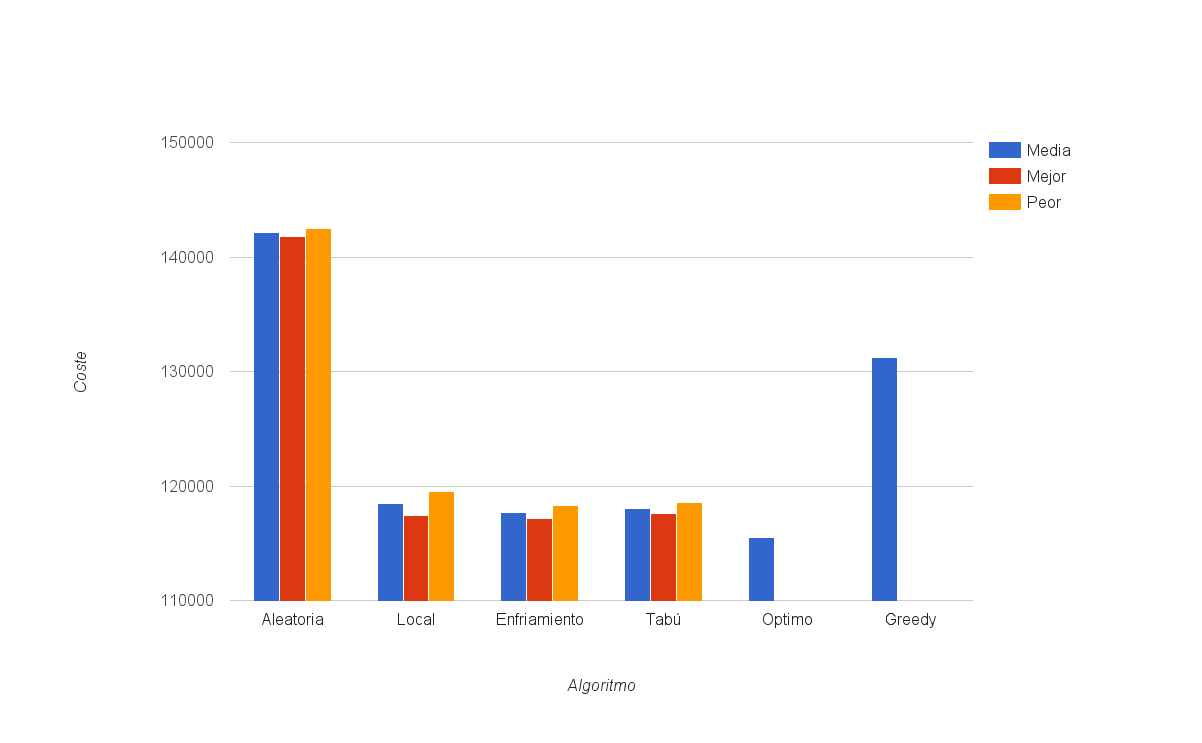
\includegraphics[scale=0.38]{./Grafico90.png}}
\caption{Resultados de los algoritmos para el problema Sko90}
\end{figure}

\begin{table}[H]
\centering
\caption{Resultados globales de los algoritmos para el problema Tai150}
\begin{tabular}{c || r | r | r | r}
Algoritmo 	& Peor & Media & Mejor & Desv. T. \\ \hline
Óptimo 		& - 	& 498896643	&	-	&	-		\\
Greedy 		& - 	& 623469733	&	-	&	-		\\ \hline
B. Aleatoria & 683620162 & 682220716 & 680849383 & \textbf{975284} \\
B. Local & 522055451 & 517687135 & 513041392 & 3103204 \\
Enf. Simu & 524200812 & 516358281 & 513226444 & 3374897 \\
B. Tabú & \quad \textbf{517545690} & \quad \textbf{512865429} & \quad \textbf{510626132} & \quad 2040887 \\
\end{tabular}
\end{table}

\begin{figure}[H]
\center
\centerline{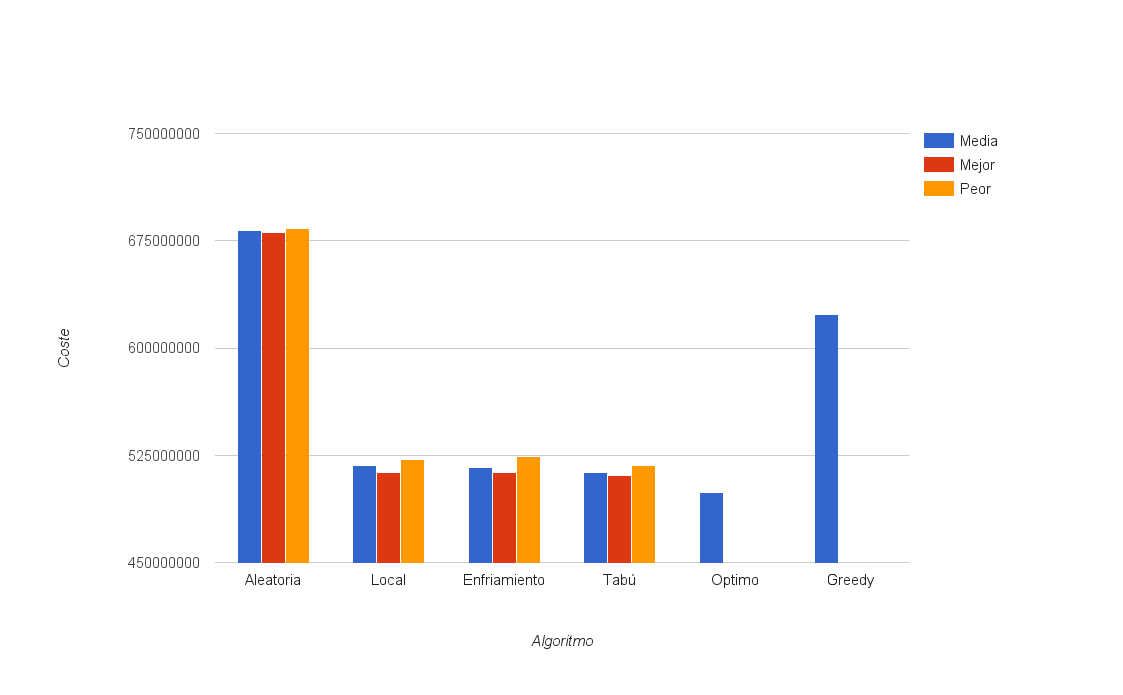
\includegraphics[scale=0.38]{./Grafico150.png}}
\caption{Resultados de los algoritmos para el problema Tai150}
\end{figure}

\section{Análisis y conclusiones}

En general, el algoritmo de Búsqueda Aleatoria obtiene peores resultados que la solución Greedy. Además de tener en todos los casos la desviación típica menor, lo que indica que no solo obtiene malos resultados sino que no suele alejarse de ellos.

Para los tres problemas estudiados el algoritmo de Búsqueda Local obtiene resultados mejores que la solución Greedy y bastante mejores que las soluciones aleatorias, pero tiene una desviación típica alta lo que indica que no es un algoritmo que de resultados sólidos.

Para el problema de tamaño 90 el Enfriamiento simulado obtiene el mejor resultado, seguido muy de cerca por el algoritmo de Búsqueda Tabú que además obtiene el mejor resultado en los otros dos problemas. 

En todos los casos, la desviación típica de los resultados de Búsqueda Tabú es inferior a la de enfriamiento simulado y búsqueda local, lo que indica que es el algoritmo más sólido de todos y tiene más probabilidad de dar una mejor solución en un menor número de ejecuciones.

En cuanto al número de iteraciones, destacar que el algoritmo de Búsqueda Tabú obtiene mejores resultado que el enfriamiento simulado habiendo realizado la mitad de iteraciones y analizando menos vecinos por iteración (40 Tabú frente a 50 enfriamiento).

En general, tanto el Enfriamiento Simulado como la Búsqueda Tabú son buenas opciones frente al resto de algoritmos para enfrentar problemas de búsqueda de grandes dimensiones, sin embargo la mejora de la Búsqueda Tabú sobre el Enfriamiento Simulado no parece demasiado significativa, sobre todo teniendo en cuenta que la implementación del algoritmo Tabú es más compleja.

\end{document}